\documentclass{beamer}

\usepackage[utf8]{inputenc}
\usepackage{listings}
\usepackage{color}
\usepackage{enumitem}
\usepackage{hyperref}
\usepackage[orientation=landscape,size=custom,width=16,height=9,scale=0.5,debug]{beamerposter}

\usepackage[ngerman]{babel}
\usepackage[ngerman]{isodate}
\usepackage[parfill]{parskip}



\usepackage[backend=bibtex,style=numeric]{biblatex}
\addbibresource{../lib/research.bib}

\usepackage{ltablex} % mix out of tabularx and longtable
\usepackage{multirow}

\usepackage{graphicx}
\usepackage{wrapfig}
\usepackage{subcaption} %To create subfigures
% \usepackage{subfig} %To create subfigures
\usepackage{placeins} % FloatBarrier
% \usepackage{floatrow}
\graphicspath{ {../images/} }

\usepackage[]{geometry}
\usepackage{pdflscape}
\usepackage{booktabs}

\usepackage[most]{tcolorbox}
\usepackage{cleveref}
\usepackage{tikz}
\usetikzlibrary{decorations.pathreplacing,shapes,arrows,positioning}
\usetikzlibrary{positioning}
\usetikzlibrary{backgrounds}
\usetikzlibrary{patterns}
\usetikzlibrary{calc}
\usetikzlibrary{fit}
\usepackage[absolute,overlay]{textpos}

\tikzstyle{input} = [coordinate]
\tikzstyle{output} = [coordinate]
\tikzstyle{block} = [rectangle, draw, text width=5em, text centered,  minimum height=4em]
\tikzstyle{storage} = [cylinder, shape border rotate=90, aspect=0.25, draw]
\tikzstyle{label} = [text width=2.4cm, text centered]
\tikzstyle{wideblock} = [rectangle, draw, text width=7em, text centered,  minimum height=4em]


\definecolor{dkgreen}{rgb}{0,0.6,0}
\definecolor{gray}{rgb}{0.5,0.5,0.5}
\definecolor{mauve}{rgb}{0.58,0,0.82}

\lstset{frame=tb,
  language=C++,
  aboveskip=3mm,
  belowskip=3mm,
  showstringspaces=false,
  columns=flexible,
  basicstyle={\small\ttfamily},
  numbers=left,
  numberstyle=\tiny\color{gray},
  keywordstyle=\color{blue},
  morekeywords={vector},
  commentstyle=\color{dkgreen},
  stringstyle=\color{mauve},
  breaklines=true,
  breakatwhitespace=true,
  tabsize=3
}



\definecolor{lmugreen}{RGB}{50,55,44}

\setbeamercolor{title}{fg=lmugreen}
\setbeamercolor{titlelike}{fg=lmugreen}
%\setbeamertemplate{itemize items}[circle]
% \setbeamertemplate{itemize items}{\color{black}$\blacktriangleright$}
%\setbeamertemplate{footline}[frame number]
\setbeamercolor{description item}{fg=black!80!black}
\setbeamerfont{description item}{size=\footnotesize}

\setbeamertemplate{footline}[text line]{%
  \parbox{\linewidth}{\vspace*{-8pt}cimarron\hfill\insertshortauthor\hfill\insertframenumber/\inserttotalframenumber}}
\setbeamertemplate{navigation symbols}{}


%Information to be included in the title page:
\title{\textbf{Cimarron}\\Stabilization of videos in modern \texttt{C++}}
\subtitle{Praktikumsabschlusspr\"asentation}
\author{Marius Herget}
\date{\today}
\institute{Institut f\"ur Informatik, LMU M\"unchen}

\usebackgroundtemplate%
{%
    
\includegraphics[width=\paperwidth,height=\paperheight]{images/bg-empty.pdf}%
}
\setbeamertemplate{frametitle}[default][center]

\newcommand{\currentSD}{}

\begin{document}

\frame{\titlepage}

\begin{frame}
\frametitle{Zielsetzung}
\begin{description}
    \item[Videostabilisierung] Methodik um ungewollte Bewegungen (Wackler) der Kamera in einem Video zu reduzieren
    \item[\texttt{C++}] eignet sich besonders gut, da Konzepte formuliert werden koennen, auf deren Grundlage eine Anwendung implementiert werden kann und die Speicherverwaltung deterministisch und minimal ist.
    \item[Ziel] Entwicklung einer Programmierabstraktion zum Kompensieren von ungewollten Bewegungen (Translation und Rotation) der Kamera mit Hilfe von Feature Tracking
\end{description}
\end{frame}

\begin{frame}
\begin{center}
    \textbf{\huge DEMO}
\end{center}
\end{frame}

\begin{frame}
    \frametitle{System Diagram}
    \begin{figure}[h!]
        \resizebox{\textwidth}{!}{%
        \begin{figure}[h!]
% \centered
\small
\begin{tikzpicture}[node distance=1cm and 2cm,auto]
    \node [input, name=input] {};
    \node [block, right= of input] (pre1) {\textbf{Decoding} Extracting frames};
    \node [block, right= of pre] (analysis1) {\textit{\tiny Local Motion Estimation:} CAMShift Tracking};
    \node [block, right= of analysis1] (analysis2) {\textit{\tiny Motion Aggregation:} CompareTrackingVectors};
    \node [block, right= of analysis2] (analysis3) {\textit{\tiny Motion Analysis:} Filter Tracking Errors};
    \node [block, below= of analysis3] (analysis3) {\textit{\tiny Global Motion Analysis:} Aggregation to global motion data};
    \node [block, left= of analysis3] (stabi) {\textit{\tiny Stabilization:} Transform frames};
    \node [block, left= of stabi] (post1) {\textit{\tiny Post-processing:} Reframe image};
    \node [block, left= of post1] (post2) {Encoding};
    \node [input, left=of post2] (output) {t};

    \node [storage, below right=0.5cm and 0.7cm of analysis] (analysisstorage) {DB};

     \draw[->](input) -- node {Video}(pre);
     \draw[->](analysis1) -- node {Motion Tracking Data}(analysis2);
     \draw[->](analysis1) -- node {\tiny Correctiondata} node[below]{m(n) = TV(n)}(analysis2);

     \draw[->](post) -- node {Video}(output);
\end{tikzpicture}
\caption{High-level system diagram}
\end{figure}
}
        \caption{High-level system diagram}
    \end{figure}
\end{frame}

\begin{frame}
\frametitle{Feature Tracking}
    \begin{columns}
    \begin{column}{0.3\textwidth}
        \begin{figure}
            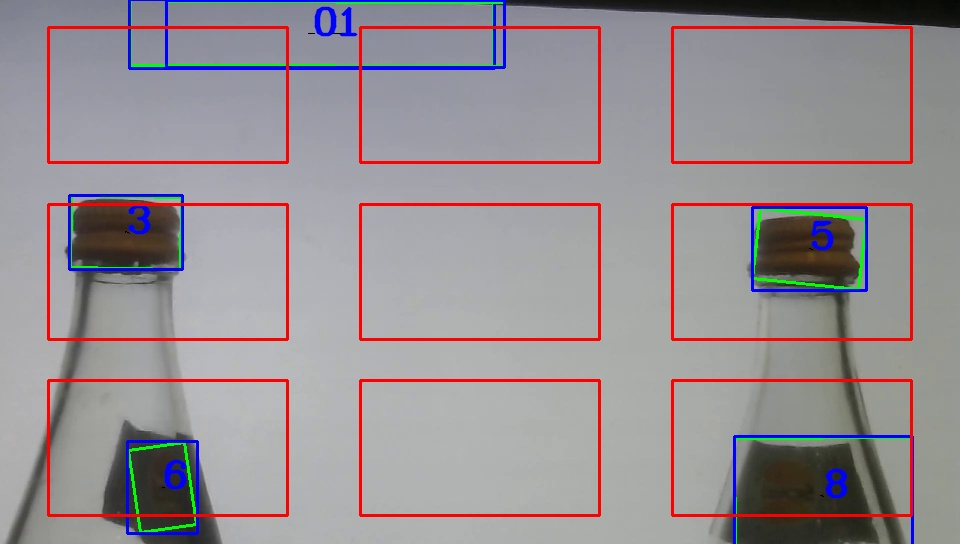
\includegraphics[scale=0.125]{tracking-example.jpg}
            \caption{Beispiel}
        \end{figure}
    \end{column}
    \begin{column}{0.67\textwidth}
            \textbf{CAMshift} Algorithmus von OpenCV \cite{OpenCVMe72:online}:\\[0.7em]
            % \begin{enumerate}
                \textbf{1.} Meanshift\\
                \textbf{2.} Fenstergroesse und Orientierung anpassen\\
                \textbf{3.} Wiederhole 1. bis gewuenschte Genauigkeit erreicht ist
            % \end{enumerate}
    \end{column}
    \end{columns}
    % SMALL SD
    \renewcommand{\currentSD}{\draw[red,thick,dotted] ($(analysis1.north west)+(-0.2,0.2)$)  rectangle ($(analysis1.south east)+(0.2,-0.2)$);}
    

\begin{textblock*}{\the\textwidth}(30pt,215pt)\centering
\resizebox{\textwidth}{!}{%
\begin{tikzpicture}[node distance=2cm and 2.55cm,auto]\centering
    \node [input, name=input] {};
    \node [block, right= of input] (pre1) {Decode};
    \node [block, right= of pre1] (analysis1) {Track};
    \node [block, right= of analysis1] (analysis2) {Compare};
    \node [block, right= of analysis2] (analysis3) {FilterErrors};
    \node [block, right= of analysis3] (analysis4) {Aggregate};
    \node [block, right= of analysis4] (stabi) {Transform \textit{(Stabilize)}};
    \node [block, right= of stabi] (post1) {Reframe};
    \node [block, right= of post1] (post2) {Encode};
    \node [input, right=of post2] (output) {t};

    \currentSD

    % \node [storage, below right=0.5cm and 0.7cm of analysis] (analysisstorage) {DB};

     \draw[->](input) -- node {Video}(pre1);
     \draw[->](pre1) -- node[label] {Frames} node[below]{$f(n)$}(analysis1);
     \draw[->](analysis1) -- node[label]{Motiondata} node[below]{$m(n)$}(analysis2);
     \draw[->](analysis2) -- node[label]{Delta Tracking} node[below]{$d(n, n+1)$}(analysis3);
     \draw[->](analysis3) -- node[label,above]{Delta Tracking} node[below]{$d(n, n+1)$}(analysis4);
     \draw[->](analysis4) -- node[label,above]{Global Delta Tracking} node[below]{$gd(n, n+1)$}(stabi);
     \draw[->](stabi) -- node[label,above]{Frames} node[below]{$f(n)$}(post1);
     \draw[->](post1) -- node[label,above]{Frames} node[below]{$f(n)$}(post2);

     \draw[->](post2) -- node[above]{Video}(output);
\end{tikzpicture}
}
\end{textblock*}

\end{frame}

\begin{frame}
\frametitle{Bewegungsmuster}
    \begin{figure}\centering
        \begin{minipage}{.45\textwidth}\centering
            \begin{tikzpicture}[scale=1]
            \draw[step=0.5cm,gray,thin] (-3,-2) grid (2,1);
            \draw[black, fill = black] (-2,-0.5) circle [radius=.5];
            \draw[black, pattern=dots] (1,-0.5) circle [radius=.5];
            \draw[thick, black, ->, line width=1mm] (-1.25,-0.5) -- node[above]{\small$\overrightarrow{v} = (6,0)$} (0.25,-0.5);
            \end{tikzpicture}
            \subcaption{Translation}
        \end{minipage}
        \begin{minipage}{.45\textwidth}\centering
            \begin{tikzpicture}[scale=1]
            \draw[step=0.5cm,gray,thin] (-3,-2) grid (2,1);

            \draw[black, fill = black]  (-2.5,0) rectangle (-1.5,-1);
            \draw[black, pattern=dots,rotate around={45:(1,-0.5)}] (0.5,0) rectangle (1.5,-1);
            % \draw[thick, black, ->, line width=1mm] (-1.25,-0.5) -- (0.15,-0.5);
            \draw[-stealth,  black, line width=0.5mm] (-1.75,0.25) arc  (100:0:0.5)node[above right]{\small$45^\circ$};
            \end{tikzpicture}
            \subcaption{Rotation}
        \end{minipage}
        % \caption{Zwei }
        \label{fig:motionmodels}
    \end{figure}
    % SMALL SD
    \renewcommand{\currentSD}{\draw[red,thick,dotted] ($(analysis2.north west)+(-0.2,0.2)$)  rectangle ($(analysis2.south east)+(0.2,-0.2)$);}
    

\begin{textblock*}{\the\textwidth}(30pt,215pt)\centering
\resizebox{\textwidth}{!}{%
\begin{tikzpicture}[node distance=2cm and 2.55cm,auto]\centering
    \node [input, name=input] {};
    \node [block, right= of input] (pre1) {Decode};
    \node [block, right= of pre1] (analysis1) {Track};
    \node [block, right= of analysis1] (analysis2) {Compare};
    \node [block, right= of analysis2] (analysis3) {FilterErrors};
    \node [block, right= of analysis3] (analysis4) {Aggregate};
    \node [block, right= of analysis4] (stabi) {Transform \textit{(Stabilize)}};
    \node [block, right= of stabi] (post1) {Reframe};
    \node [block, right= of post1] (post2) {Encode};
    \node [input, right=of post2] (output) {t};

    \currentSD

    % \node [storage, below right=0.5cm and 0.7cm of analysis] (analysisstorage) {DB};

     \draw[->](input) -- node {Video}(pre1);
     \draw[->](pre1) -- node[label] {Frames} node[below]{$f(n)$}(analysis1);
     \draw[->](analysis1) -- node[label]{Motiondata} node[below]{$m(n)$}(analysis2);
     \draw[->](analysis2) -- node[label]{Delta Tracking} node[below]{$d(n, n+1)$}(analysis3);
     \draw[->](analysis3) -- node[label,above]{Delta Tracking} node[below]{$d(n, n+1)$}(analysis4);
     \draw[->](analysis4) -- node[label,above]{Global Delta Tracking} node[below]{$gd(n, n+1)$}(stabi);
     \draw[->](stabi) -- node[label,above]{Frames} node[below]{$f(n)$}(post1);
     \draw[->](post1) -- node[label,above]{Frames} node[below]{$f(n)$}(post2);

     \draw[->](post2) -- node[above]{Video}(output);
\end{tikzpicture}
}
\end{textblock*}

\end{frame}
\note[itemize]{
\item Perspektive fehlt: Kann man aber implementieren ueber die Groesse des Tracking Windows und abhangigkeiten von den TVs: Inverse ist berechnbar
}

\begin{frame}
\frametitle{Bewegungserkennung}
    \begin{description}
        \item[Lokal] $\Delta(trackingVector(F(n-1)), trackingVectorF(n))$
        \item[Global]
    \end{description}
    % SMALL SD
    \renewcommand{\currentSD}{\draw[red,thick,dotted] ($(analysis2.north west)+(-0.2,0.4)$)  rectangle ($(analysis4.south east)+(0.2,-0.4)$);}
    

\begin{textblock*}{\the\textwidth}(30pt,215pt)\centering
\resizebox{\textwidth}{!}{%
\begin{tikzpicture}[node distance=2cm and 2.55cm,auto]\centering
    \node [input, name=input] {};
    \node [block, right= of input] (pre1) {Decode};
    \node [block, right= of pre1] (analysis1) {Track};
    \node [block, right= of analysis1] (analysis2) {Compare};
    \node [block, right= of analysis2] (analysis3) {FilterErrors};
    \node [block, right= of analysis3] (analysis4) {Aggregate};
    \node [block, right= of analysis4] (stabi) {Transform \textit{(Stabilize)}};
    \node [block, right= of stabi] (post1) {Reframe};
    \node [block, right= of post1] (post2) {Encode};
    \node [input, right=of post2] (output) {t};

    \currentSD

    % \node [storage, below right=0.5cm and 0.7cm of analysis] (analysisstorage) {DB};

     \draw[->](input) -- node {Video}(pre1);
     \draw[->](pre1) -- node[label] {Frames} node[below]{$f(n)$}(analysis1);
     \draw[->](analysis1) -- node[label]{Motiondata} node[below]{$m(n)$}(analysis2);
     \draw[->](analysis2) -- node[label]{Delta Tracking} node[below]{$d(n, n+1)$}(analysis3);
     \draw[->](analysis3) -- node[label,above]{Delta Tracking} node[below]{$d(n, n+1)$}(analysis4);
     \draw[->](analysis4) -- node[label,above]{Global Delta Tracking} node[below]{$gd(n, n+1)$}(stabi);
     \draw[->](stabi) -- node[label,above]{Frames} node[below]{$f(n)$}(post1);
     \draw[->](post1) -- node[label,above]{Frames} node[below]{$f(n)$}(post2);

     \draw[->](post2) -- node[above]{Video}(output);
\end{tikzpicture}
}
\end{textblock*}

\end{frame}

\begin{frame}
\frametitle{Stabilisierung Theorie}
    \begin{figure}\centering
        \begin{minipage}{.45\textwidth}\centering
            \begin{tikzpicture}[scale=1]
            \draw[step=0.5cm,gray,thin] (-3,-2) grid (2,1);
            \draw[black, fill = black] (-2,-0.5) circle [radius=.5];
            \draw[black, pattern=dots] (1,-0.5) circle [radius=.5];
            \draw[thick, black, ->, line width=1mm] (-1.25,-0.5) -- node[above]{\small$\overrightarrow{v} = (6,0)$} (0.25,-0.5);
            \draw[thick, white, ->, line width=0.001mm] (-1.25,1.1) -- node[above]{\small$\overrightarrow{v} = (6,0)$} (-2.75,1.1);
            \end{tikzpicture}
            \subcaption{Erkennung}
        \end{minipage}
        \begin{minipage}{.45\textwidth}\centering
            \begin{tikzpicture}[scale=1]
            \draw[step=0.5cm,gray,thin] (-3,-2) grid (2,1);
            \draw[black, fill = gray] (-2,-0.5) circle [radius=.5];
            \draw[thick, blue, ->, line width=0.5mm] (-1.25,1.1) -- node[above]{\small$\overrightarrow{v} = (-6,0)$} (-2.75,1.1);

            \draw[step=0.5cm,blue,thin] (-5,-2) grid (-1,1);
            \draw[blue, pattern=dots] (-2,-0.5) circle [radius=.5];


            \end{tikzpicture}
            \subcaption{Inverse}
        \end{minipage}
        \caption{Translationsstabilisierung}
        \label{fig:motionmodels}
    \end{figure}
    % SMALL SD
    \renewcommand{\currentSD}{\draw[red,thick,dotted] ($(stabi.north west)+(-0.2,0.2)$)  rectangle ($(stabi.south east)+(0.2,-0.2)$);}
    

\begin{textblock*}{\the\textwidth}(30pt,215pt)\centering
\resizebox{\textwidth}{!}{%
\begin{tikzpicture}[node distance=2cm and 2.55cm,auto]\centering
    \node [input, name=input] {};
    \node [block, right= of input] (pre1) {Decode};
    \node [block, right= of pre1] (analysis1) {Track};
    \node [block, right= of analysis1] (analysis2) {Compare};
    \node [block, right= of analysis2] (analysis3) {FilterErrors};
    \node [block, right= of analysis3] (analysis4) {Aggregate};
    \node [block, right= of analysis4] (stabi) {Transform \textit{(Stabilize)}};
    \node [block, right= of stabi] (post1) {Reframe};
    \node [block, right= of post1] (post2) {Encode};
    \node [input, right=of post2] (output) {t};

    \currentSD

    % \node [storage, below right=0.5cm and 0.7cm of analysis] (analysisstorage) {DB};

     \draw[->](input) -- node {Video}(pre1);
     \draw[->](pre1) -- node[label] {Frames} node[below]{$f(n)$}(analysis1);
     \draw[->](analysis1) -- node[label]{Motiondata} node[below]{$m(n)$}(analysis2);
     \draw[->](analysis2) -- node[label]{Delta Tracking} node[below]{$d(n, n+1)$}(analysis3);
     \draw[->](analysis3) -- node[label,above]{Delta Tracking} node[below]{$d(n, n+1)$}(analysis4);
     \draw[->](analysis4) -- node[label,above]{Global Delta Tracking} node[below]{$gd(n, n+1)$}(stabi);
     \draw[->](stabi) -- node[label,above]{Frames} node[below]{$f(n)$}(post1);
     \draw[->](post1) -- node[label,above]{Frames} node[below]{$f(n)$}(post2);

     \draw[->](post2) -- node[above]{Video}(output);
\end{tikzpicture}
}
\end{textblock*}

\end{frame}
%
\begin{frame}
\frametitle{Stabilisierung Theorie}
\vspace{-1.2em}
    \begin{figure}\centering
        \begin{minipage}{.4\textwidth}\centering
            \begin{tikzpicture}[scale=1]
            \draw[step=0.5cm,gray,thin] (-3,-2) grid (2,1);

            \draw[black, fill = black]  (-2.5,0) rectangle (-1.5,-1);
            \draw[black, pattern=dots,rotate around={45:(1,-0.5)}] (0.5,0) rectangle (1.5,-1);
            % \draw[thick, black, ->, line width=1mm] (-1.25,-0.5) -- (0.15,-0.5);
            \draw[-stealth,  black, line width=0.5mm] (-1.75,0.25) arc  (100:0:0.5)node[above right]{\small$45^\circ$};
            \end{tikzpicture}
            \subcaption{Erkennung}
        \end{minipage}
        \begin{minipage}{.58\textwidth}\centering
            \begin{tikzpicture}[scale=1]
            \draw[step=0.5cm,gray,thin] (-3,-2) grid (2,1);
            \draw[step=0.5cm,blue,rotate around={45:(1,-0.5)},thin] (-3,-2) grid (2,1);

            \draw[black, fill = black]  (-2.5,0) rectangle (-1.5,-1);
            \draw[blue, pattern=dots,] (0.5,0) rectangle (1.5,-1);
            % \draw[thick, black, ->, line width=1mm] (-1.25,-0.5) -- (0.15,-0.5);
            \draw[-stealth,  blue, line width=0.5mm] (-2.7,-1.8) arc  (80:275:0.5)node[below left]{\small$-45^\circ$};
            \end{tikzpicture}
            \subcaption{Inverse}
        \end{minipage}
% \protect\caption[position=left]{Rotationsstabilisierung}
        % {\hspace*{-2em}\caption{Rotationsstabilisierung}}
        \label{fig:motionmodels}
    \end{figure}
    % SMALL SD
    \renewcommand{\currentSD}{\draw[red,thick,dotted] ($(stabi.north west)+(-0.2,0.2)$)  rectangle ($(stabi.south east)+(0.2,-0.2)$);}
    

\begin{textblock*}{\the\textwidth}(30pt,215pt)\centering
\resizebox{\textwidth}{!}{%
\begin{tikzpicture}[node distance=2cm and 2.55cm,auto]\centering
    \node [input, name=input] {};
    \node [block, right= of input] (pre1) {Decode};
    \node [block, right= of pre1] (analysis1) {Track};
    \node [block, right= of analysis1] (analysis2) {Compare};
    \node [block, right= of analysis2] (analysis3) {FilterErrors};
    \node [block, right= of analysis3] (analysis4) {Aggregate};
    \node [block, right= of analysis4] (stabi) {Transform \textit{(Stabilize)}};
    \node [block, right= of stabi] (post1) {Reframe};
    \node [block, right= of post1] (post2) {Encode};
    \node [input, right=of post2] (output) {t};

    \currentSD

    % \node [storage, below right=0.5cm and 0.7cm of analysis] (analysisstorage) {DB};

     \draw[->](input) -- node {Video}(pre1);
     \draw[->](pre1) -- node[label] {Frames} node[below]{$f(n)$}(analysis1);
     \draw[->](analysis1) -- node[label]{Motiondata} node[below]{$m(n)$}(analysis2);
     \draw[->](analysis2) -- node[label]{Delta Tracking} node[below]{$d(n, n+1)$}(analysis3);
     \draw[->](analysis3) -- node[label,above]{Delta Tracking} node[below]{$d(n, n+1)$}(analysis4);
     \draw[->](analysis4) -- node[label,above]{Global Delta Tracking} node[below]{$gd(n, n+1)$}(stabi);
     \draw[->](stabi) -- node[label,above]{Frames} node[below]{$f(n)$}(post1);
     \draw[->](post1) -- node[label,above]{Frames} node[below]{$f(n)$}(post2);

     \draw[->](post2) -- node[above]{Video}(output);
\end{tikzpicture}
}
\end{textblock*}

\end{frame}

\begin{frame}
\frametitle{Ähnlichkeit}
\begin{description}
    \item[Vektoren] Kosinus-Ähnlichkeit
    \[cos\_sim = \frac{A \cdot B}{\Vert A\Vert \Vert B\Vert} = \frac{\sum\limits_{i=1}^{n} A_iB_i}{\sqrt{\sum\limits_{i=1}^{n}A_i^2} \sqrt{\sum\limits_{i=1}^{n}B_i^2}}\]
    \item[Winkel] Prozentuale Veraenderung
\end{description}
\end{frame}
\note[itemize]{
\item Kosinus-Ähnlichkeit ist ein Maß für die Ähnlichkeit zweier Vektoren
\item Kosinus des Winkels zwischen beiden Vektoren
\item 1:  Abhängigkeit // 0: Unabhängigkeit // -1: Exakt gegenteil
\item $[-1\leq cos\_sim \leq,1]$
\item  Attribut-Vektoren a {\displaystyle \mathbf {a} } \mathbf {a} und b {\displaystyle \mathbf {b} } \mathbf{b}
\item Der Kosinus zweier Vektoren bestimmt sich aus dem Standardskalarprodukt: $a\cdot b = \Vert A\Vert\Vert B\Vert cos \Theta$\\[1.5em]
\item $A \cdot B$ -> Skalarprodukt
\item $A \cdot B$ -> Norm:  Abbildung die dem Vektor eine Zahl zuordnet, die auf gewisse Weise die Größe des Objekts beschreiben soll
}

\begin{frame}
\frametitle{Berechnung Inverse}
    \textbf{Vektoren}:
    % \begin{enumerate}
        % \item
        Berechne die Cosine similarity von jedem Tracking window mit jedem anderen TrackingVector:
        \[cos\_sim(\forall transVector(delta(f(n), f(n+1))) )\]
    % \end{enumerate}
\end{frame}

\begin{frame}
\frametitle{Konzepte}
\end{frame}

\begin{frame}
\frametitle{Konzeptdefinition}
\end{frame}


\begin{frame}
\begin{center}
    \textbf{\huge BACKUP}
\end{center}
\end{frame}

\begin{frame}
    \frametitle{CamShift}
    \begin{figure}[h!]
        \resizebox{\textwidth}{!}{%
        
    \tcbox[enhanced, sharp corners, boxsep=1mm, boxrule=1mm,colframe=gray!10!white,
        colback=white,
        borderline={2pt}{-1pt}{gray,dotted}]
        {\begin{tikzpicture}[scale=0.6,node distance=1cm and 2.5cm,auto]
            \node [input, name=input] {};
            \node [block, right= of input] (pre1) {Initialize tracking areas};
            \node [wideblock, right= of pre1] (pre2) {Histogram \& Backprojection};
            \node [block, right= of pre2] (pre3) {Normali-sation};
            \node [block, below= of pre3] (pre4) {Mean-Shift};
            \node [wideblock, left= of pre4] (pre5) {Adjust size of tacking area and rotation};
            \node [input, left=of pre5] (output) {t};

            \draw[->](input) -- node[label]{Frames}node[below]{$f(n)$}(pre1);
            \draw[->](pre1) -- node[label]{Frames}node[below]{$f(n)$}(pre2);


            \draw[->](pre2) -- node[label]{$bj(f(n))$}node[below]{$hsv(f(n))$}(pre3);

            \draw[->](pre3) -- node[label, left]{$bj(f(n))$}node[right]{$hsv(f(n))$}(pre4);


            \draw[->](pre4) -- node[label, above]{Tackwindow}node[below]{$tv(f(n), ta)$}(pre5);
            \draw[->](pre5)  |- ++(0,-3cm) --node[label, above]{Tackwindow}node[below]{$tv(f(n), ta)$} ++(8.875cm,0) -- (pre4);


            \draw[->](pre5) -- node[label, above]{Motiondata}node[below]{$m(n)$}(output);
        \end{tikzpicture}
        }
}
        \caption{Detailed system diagram of \textit{Track}}
    \end{figure}
\end{frame}

\end{document}
